\newline
\newline
\vspace{3mm}
\hfill
\section{Introduction}
\hspace{2cm}In this chapter we will rather take a higher approach to our system, introducing our main software platform (ROS), which is considered as the beating heart of our system, then we illustrate the flow of data between the various system components. For the rest of this chapter we introduce our work environment on Raspberry Pi 3.

\section{Robot Operating System (ROS)}

\subsection{Introduction to ROS}
\hspace{2cm}ROS is an open source meta-operating system that runs on Unix operating systems, such as Linux Ubuntu. Similar to a regular operating system, it can provide low-level device control and message-passing between processes, but it is not designed to be the main operating system of a device. Since ROS is open source, it includes many online repositories from other organizations or community of developers, including industrial applications. ROS run-time graph is a peer-to-peer network of processes (potentially distributed across machines) that are loosely coupled using the ROS communication infrastructure. ROS implements several different styles of communication, including synchronous RPC-style communication over services, asynchronous streaming of data over topics, and storage of data on a Parameter Server.\cite{web040}

\begin{figure}[H]%
    \center%
    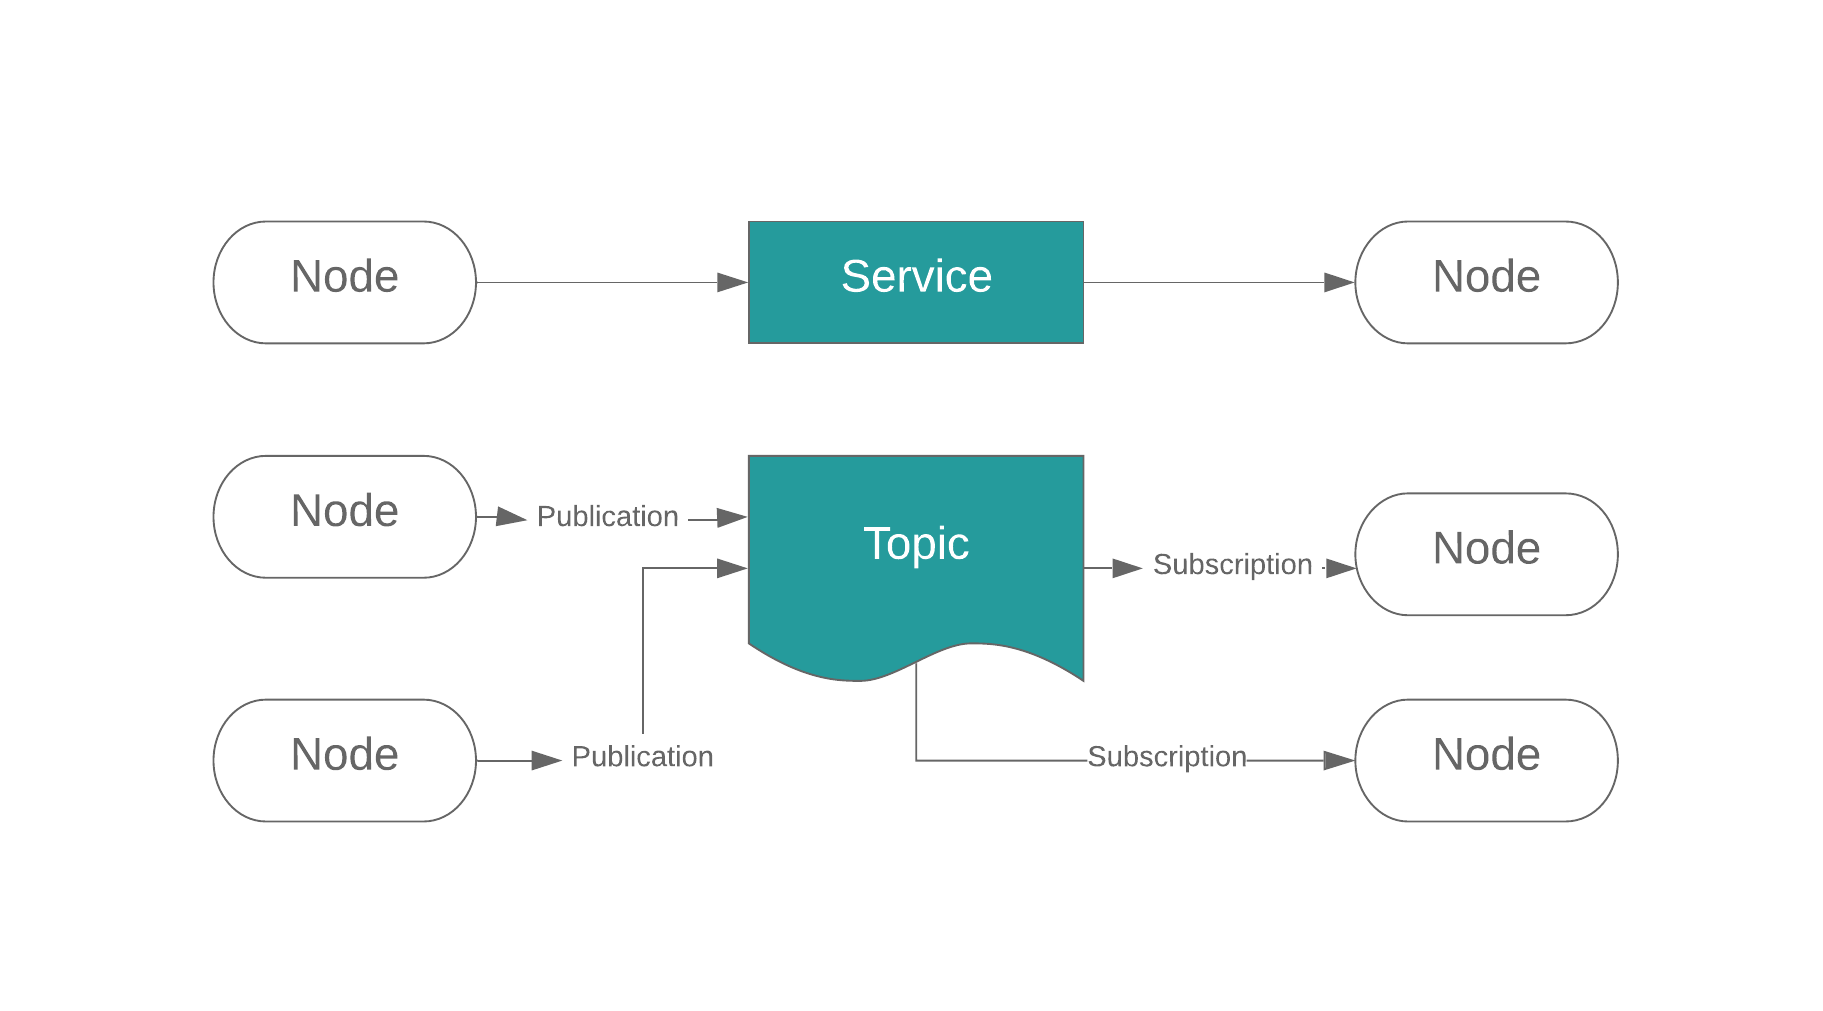
\includegraphics[width=1\textwidth]{images/Dada/RosNodesandTopics.png}%
     % you need to add the caption for the list of figures
    \caption[ROS Nodes and Topics]{ROS Nodes and Topics}\label{fig: ROS Nodes and Topics}%
  \end{figure}
  
\subsection{ROS Nodes, Topics, and Messages}
\hspace{2cm}ROS nodes are processes that usually does some computation and are able to
communicate with each other. Some examples for this experiment are one node responsible for the IMU data, another node responsible for the Gps data, and another node responsible for processing both sensor data. They can communicate through the use of topics. In order for nodes to communicate, a unique topic, service, or server name must be assigned by the node. Afterwards, any node in the system can publish or subscribe to that topic name. Publishing to a topic is similar to sending data to that topic name, while subscribing is similar to receiving the data. Each topic must be assigned a proper message structure, either custom built or one of the ROS messages. For example, there is an already built ROS message for IMU that contains linear acceleration, angular velocity, and orientation data. It is important to note that the node publishing and subscribing to the topic must use the same message structure.\cite{web040}

\section{Data Flow Abstraction}
\hspace{2cm}In this section we will illustrate the flow of the data inside the main device (Raspberry Pi), that resides and drives the robot. The flow of data inside the main controller is as shown in fig \ref{fig: Main Controller Data Flow Diagram}.
\subsection{Data Flow Diagram}
\hspace{2cm}The main controller consists of the following modules:
\begin{enumerate}
    \item Task handler Module 
    \item Classical Controller Module
    \item Obstacle Avoidance Module
    \item Main controller Module
    \item Serial Communication Module
\end{enumerate}
\subsubsection{Task Handler Module }
\hspace{2cm}The Task handler module is a ROS node that contains a web server. The server receives the incoming HTTP POST requests, which contains the task data, Processing the data and generating a sequence of sub-tasks, each sub-task contains a position and a flag that defines if the classical controller or the Module should take control at that point, Finally publishing that task on a ROS topic.
\begin{figure}[H]%
    \center%
    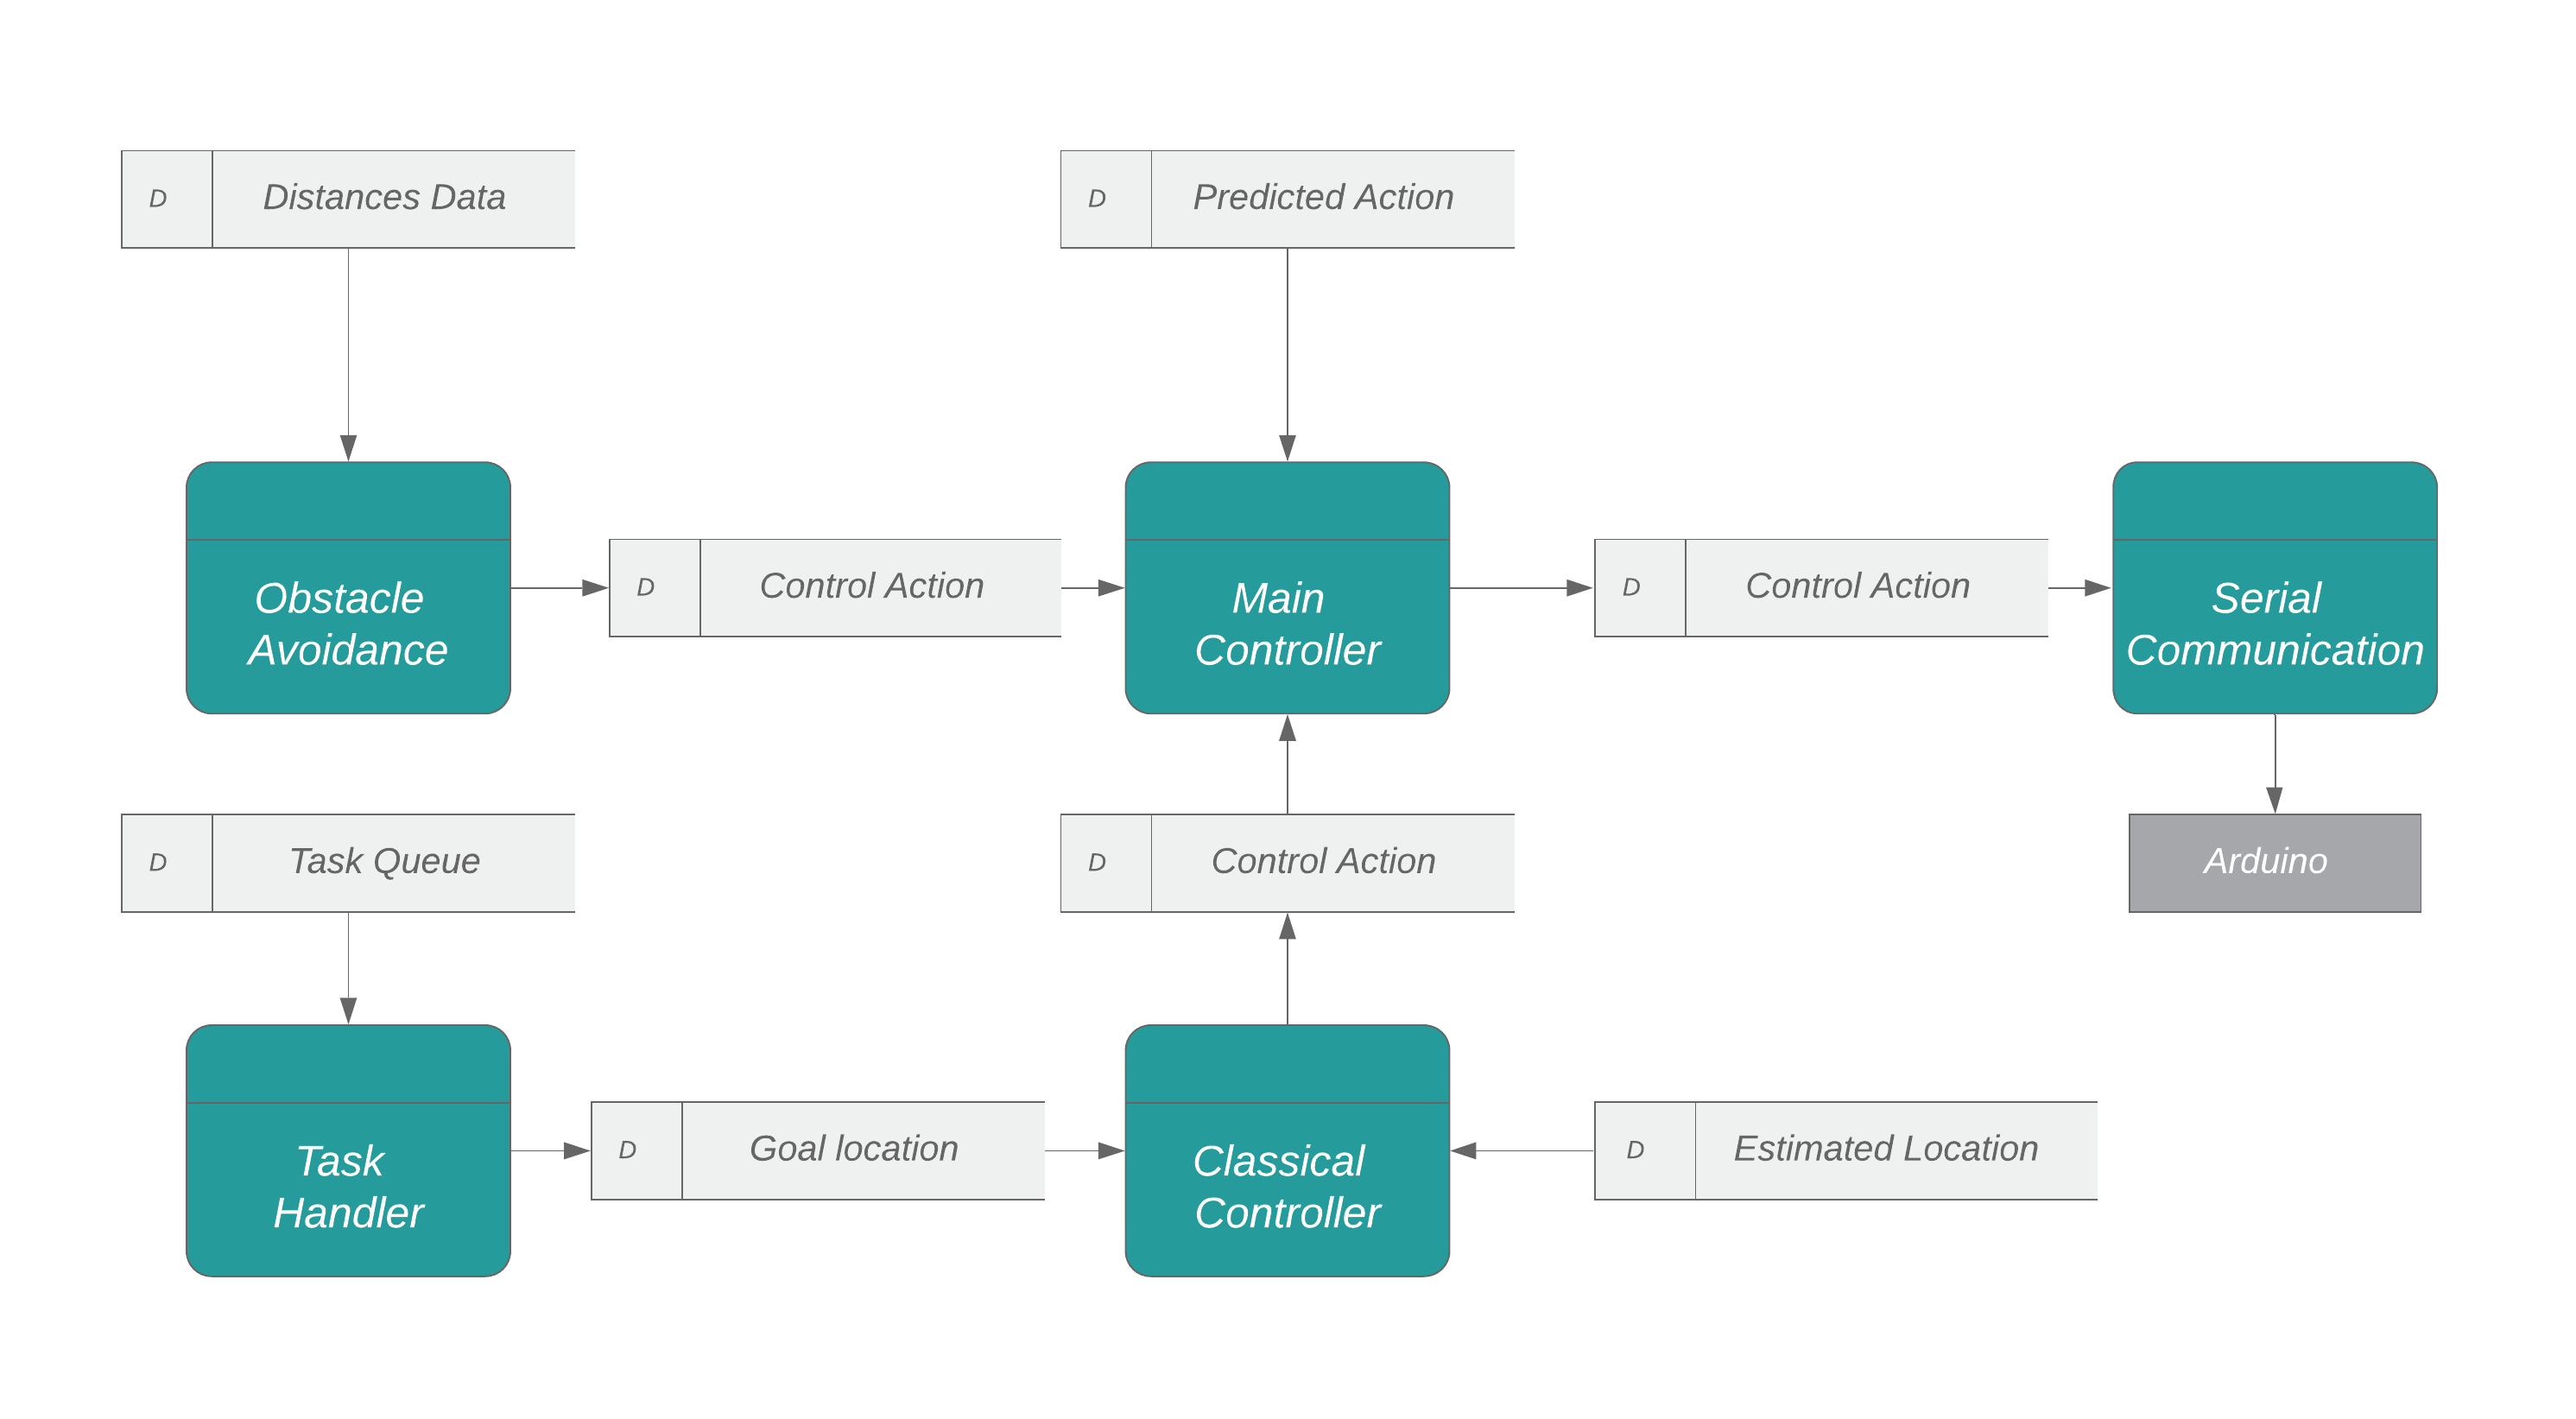
\includegraphics[width=.8\textwidth]{images/Dada/DataFlowDiagram.png}%
     % you need to add the caption for the list of figures
    \caption[Main Controller Data Flow Diagram]{Main Controller Data Flow Diagram}\label{fig: Main Controller Data Flow Diagram}%
  \end{figure}
\subsubsection{Classical Controller Module}
\hspace{2cm}The Classical Controller module is a ROS node, which takes the current location (estimated location from the localization module over a socket connection) and, the goal location ( provided from the task handler),  processing both location and generating the suitable control action to move the robot from the current location to the goal location
\subsubsection{Obstacle Avoidance Module}
\hspace{2cm}The Obstacle Avoidance module is a ROS node, which subscribes to the LIDAR data topic containing ranges and distances, then if the distance is below a certain threshold it outputs a high-priority control action, that is sent to the main controller.
\subsubsection{Main Controller Module}
 \hspace{2cm}The main controller is a ROS node that takes in all the control actions from the    Module, the obstacle avoidance module and the classical controller and based on the current information provided from the task handler, chooses which control action is sent to the serial communication module.
\subsubsection{Serial Communication Module}
\hspace{2cm}The Serial Communication module is a ROS Node that subscribes to the control action topic published from the main controller and then send it to the Arduino using serial port communication.

\section{Robot Work Environment}
\hspace{2cm}In this section we describe the main device environment on the robot. This main device communicates with the various components of the robot, after processing the data collected from them, it sends the appropriate control action to drive the actuators through the Arduino. We used The Nvidia Jetson TX1 development kit as our main computer, mainly because of it's computation capability, but due to some technical issues we were forced to downgrade to The Rasbpery pi model 3. The full hardware specification of the Rasbperry pi we used are on chapter 2.

\subsection{Raspberry Pi}
\hspace{2cm}In chapter 2 we covered the hardware specification of the Raspberry Pi we are using, we now introduce our work environment on the Raspberry Pi. We are using ROSbots \cite{web024}, which is Raspbian Stretch lite (Debian-based computer operating system for Raspberry Pi provided by the Raspberry Pi Foundation\cite{web025}) equipped with ROS Kinetic\cite{web026} and OpenCV  pre-installed on it.

\subsection{Operating ROS on The Raspberry Pi}
\hspace{2cm}The ROS Environment or ROS Work-space (as in ROS terms) on the Raspberry Pi consists of four essential packages:

\subsubsection{Sensors Package}
\hspace{2cm}Data acquisition package, It collects data from the sensors and, publishes each sensor's data to it's corresponding ROS Topic, So it could be used by other Nodes by subscribing to that topic.
\begin{enumerate}
    \item \textbf{IMU Node}\newline
        ROS Publisher Node that collects IMU data: Linear velocity and angular orientation and publishes this data on the IMU topic.
    \item \textbf{GPS Node}\newline
        ROS Publisher Node that collects GPS data: Longitude and latitude and, publishes this data on the GPS topic.
    \item \textbf{Camera Node}\newline
        ROS Publisher Node that collects Camera data: raw images and publishes this data on the Camera topic.
\end{enumerate}

\subsubsection{Control Package}
\hspace{2cm}The Control package is mainly used to generate control action that is published to the control action topic, whether it's generated while driving the robot manually or, while the robot is being driven autonomously by the NN model.
\begin{enumerate}
    \item \textbf{Keyboard Node}\newline
    ROS Publisher Node that generates control action in response  to the keys being pressed by the keyboard while manually driving the robot to collect data for model training.
    \item \textbf{Autopilot Node}\newline
    ROS Publisher Node that subscribes to the Camera Topic, pass the image through the NN model, Then publishing the predicted control action on the control action topic.
\end{enumerate}

\subsubsection{Communication Package}
\hspace{2cm}Communication Package contains nodes that send data from the main device to other devices or modules of the system. Through serial port communication with the Arduino, or Socket connection with the localization module.
\begin{enumerate}
    \item \textbf{Serial Node}\newline
        ROS Listener Node that subscribes to the control action topic, Continuously sending the control action to the Arduino Uno over an open serial port communication.
    \item \textbf{Data Collector Node}\newline
        ROS Listener Node that subscribes to both camera and control action topics, store both of them in an object-like data, then saves the collected data to the hard disk to be used for NN model training later.
    \item \textbf{Socket Server Node}\newline
        ROS Listener Node that subscribes to sensors topics: IMU and GPS, also the control action topic, then send them to the Localization module (socket client) through open server-client socket connection.
\end{enumerate}

\subsubsection{Web Server Package}
\hspace{2cm}Web Server Package is considered to be the bridge between the main system's web server and the ROS environment on the robot.

\begin{enumerate}
    \item \textbf{Task Handler Node}\newline
    ROS Publisher Node that contains a python web server, Capable of Handling the incoming HTTP requests that contain the task's data, Processing that data and publishing it to the task topic.
\end{enumerate}